\subsection{Application I/O Interface}\label{subsec:Application_IO_Interface}
The \nameref{def:Operating_System} wants to treat all I/O devices in a standard, uniform way.
Like other complex software-engineering problems, the approach here involves abstraction, encapsulation, and software layering.
Specifically, we can abstract away the detailed differences in I/O devices by identifying a few general kinds, where each is accessed through a standardized set of functions, its \emph{interface}.
The implementation differences are encapsulated in \nameref{def:Kernel_Module}s called \nameref{def:Device_Driver}s that internally are custom-tailored to specific devices but that export one of the standard interfaces.
The software layering used is shown in \Cref{fig:Kernel_IO_Subsystem_Structure}.

\begin{figure}[h!tbp]
  \centering
  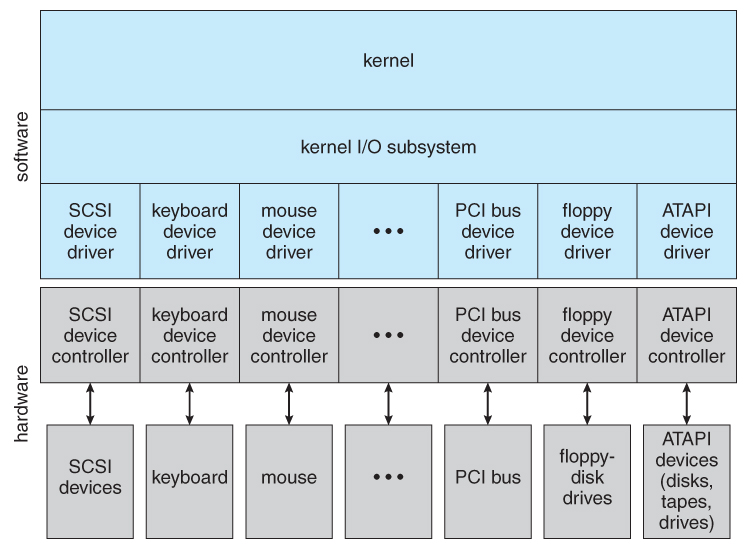
\includegraphics[scale=1.00]{./Drawings/EDAF35-Operating_Systems/Kernel_IO_Subsystem_Structure.jpg}
  \caption{Kernel I/O Subsystem Structure}
  \label{fig:Kernel_IO_Subsystem_Structure}
\end{figure}

This layering methodology is used to hide differences among devices and their controllers from the \nameref{def:Kernel}'s I/O subsystem.
This is analogous to the I/O system calls encapsulating the behavior of devices in a few generic classes that hide hardware differences from applications.

Making the I/O subsystem independent of the hardware simplifies the job of the operating-system developer.
It also benefits the hardware manufacturers.
They either:
\begin{itemize}[noitemsep]
\item Design new devices to be compatible with an existing host controller interface.
\item Write device drivers to interface the new hardware to popular operating systems.
\end{itemize}

Thus, we (users) can attach new peripherals to a computer without waiting for the operating system to develop explicit kernel-level support code.
Unfortunately for hardware manufacturers, each operating system has its own standards for the device-driver interface.

Devices can vary in many dimensions, as seen in \Cref{tab:Characteristics_IO_Devices}.
\begin{table}[h!tbp]
  \centering
  \begin{tabular}{cll}
    \toprule
    \textbf{Aspect} & \textbf{Variation} & \textbf{Example} \\
    \midrule
    \multirow{2}{*}{Data-Transfer Mode} & Character & Terminal \\
                    & Block & Disk \\
    \multirow{2}{*}{Access Method} & Sequential & Modem/Network \\
                    & Random & Magnetic Disk \\
    \multirow{2}{*}{Transfer Schedule} & Synchronous & Magnetic Tape \\
                    & Asynchronous & Keyboard \\
    \multirow{2}{*}{Sharing} & Dedicated & Magnetic Tape \\
                    & Sharable & Keyboard \\
    \multirow{4}{*}{Device Speed} & Latency & \\
                    & Seek Time & \\
                    & Transfer Rate & \\
                    & Delay between Operations & \\
    \multirow{3}{*}{I/O Direction} & & \\
                    & Read-only & CD-ROM (After first write) \\
                    & Write-only & Graphics Controller \\
                    & Read-write & Disk \\
    \bottomrule
  \end{tabular}
  \caption{Characteristics of I/O Devices}
  \label{tab:Characteristics_IO_Devices}
\end{table}

Now, each of the entries in \Cref{tab:Characteristics_IO_Devices} are further explained:
\begin{itemize}[noitemsep]
\item Character-stream or block.
  \begin{itemize}[noitemsep]
  \item Character-stream device transfers \textbf{bytes} one-by-one.
  \item A block device transfers a block of bytes as a unit.
\end{itemize}

\item Sequential or random access.
  \begin{itemize}[noitemsep]
  \item Sequential devices transfer data in a fixed order determined by the device
  \item Random-access devices can instruct the device to seek to any of the available data storage locations.
\end{itemize}

\item Synchronous or asynchronous.
  \begin{itemize}[noitemsep]
  \item Synchronous devices performs data transfers with predictable response times, in coordination with other aspects of the system.
  \item Asynchronous devices exhibits irregular or unpredictable response times not coordinated with other computer events.
\end{itemize}

\item Sharable or dedicated.
  \begin{itemize}[noitemsep]
  \item A sharable device can be used concurrently by several \nameref{def:Process}es or \nameref{def:Thread}s.
  \item Dedicated devices cannot be shared by several concurrent \nameref{def:Process}es or \nameref{def:Thread}s.
\end{itemize}

\item Speed of operation.
  Device speeds range over a wide range of speeds, from a few bytes per second to several gigabytes per second.

\item Read–write, read only, or write only.
  Some devices perform both input and output, but others support only one data transfer direction.
\end{itemize}

For the purpose of application access, many of these differences are hidden by the operating system, and the devices are grouped into a few conventional types.
\begin{itemize}[noitemsep]
\item Block I/O.
\item Character-stream I/O.
\item \nameref{subsec:Memory_Mapped_Files} access.
\item Network sockets.
\item Operating systems also provide special system calls to access a few additional devices:
  \begin{itemize}[noitemsep]
  \item Time-of-day clock.
  \item Timer.
\end{itemize}

\item Some operating systems provide a set of \nameref{def:System_Call}s for graphical display, video, and audio devices.
\end{itemize}

Most operating systems also have back door that transparently passes arbitrary commands from an application to a device driver.
In \textsc{unix}, this system call is \kernelinline{ioctl()} (for ``I/O control'').
The \kernelinline{ioctl()} \nameref{def:System_Call} enables an application to access \textbf{any} functionality that can be implemented by \textbf{any} device driver, \textbf{without} the need to invent a new system call.
The ioctl() system call has three arguments.
\begin{enumerate}[noitemsep]
\item File descriptor that connects the application to the driver by referring to a hardware device managed by that driver.
\item Integer that selects one of the commands implemented in the driver.
\item Pointer to an arbitrary data structure in memory that enables the application and driver to communicate any necessary control information or data.
\end{enumerate}

\subsubsection{Block and Character Devices}\label{subsubsec:Block_Char_Devices}
The block-device interface captures all the aspects necessary for accessing disk drives and other block-oriented devices.
The \nameref{def:Device_Driver} is expected to understand the commands:
\begin{enumerate}[noitemsep]
\item \kernelinline{read()}
\item \kernelinline{write()}
\item \kernelinline{seek()}
  \begin{itemize}[noitemsep]
  \item Only if it is a random-access device.
  \item Specifies which block to transfer next.
  \end{itemize}
\end{enumerate}

Applications normally access such these devices through the \nameref{sec:FS_Interface}.
Thus, these three functions capture the essential behaviors of block-storage devices, insulating applications from low-level differences among those devices.

The character-stream interface captures all the aspects necessary for accessing byte-by-byte generating devices.
The \nameref{def:Device_Driver} is expected to export the following commands:
\begin{enumerate}[noitemsep]
\item \kernelinline{get()}
\item \kernelinline{put()}
\end{enumerate}

This style of access is convenient for input devices (such as keyboards) that produce data for input ``spontaneously''(at times that cannot necessarily be predicted by the application).
This access style is also good for output devices such as printers and audio boards, which naturally fit the concept of a linear stream of bytes.

\paragraph{Raw I/O and Block and Character Devices}\label{par:Raw_IO_Block_Char_Devices}
The operating system itself, as well as special applications, may prefer to access a block device as a simple linear array of blocks.
This mode of access is called raw I/O.
To avoid conflicts, raw-device access passes control of the device directly to the application, letting the operating system step out of the way.
A compromise between raw I/O and file system I/O, that is becoming common, is for the operating system to allow a mode of operation on a file that disables buffering and locking.
In the \textsc{unix} world, this is called direct I/O.

\paragraph{Memory-Mapped Files and Block and Character Devices}\label{par:Memory_Mapped_Files_Block_Char_Devices}
\nameref{subsec:Memory_Mapped_Files} and their access can be layered on top of block-device drivers.
Rather than offering read and write operations, a memory-mapped interface provides access to disk storage via an array of bytes in main memory.
The \nameref{def:System_Call} that maps a \nameref{def:File} into memory returns the \nameref{def:Virtual_Memory} address that contains a \textbf{copy} of the file.
The actual data transfers are performed only when needed to satisfy access to the memory image.

The transfers are handled by the same mechanism as that used for \nameref{def:Demand_Paging} \nameref{def:Virtual_Memory} access, making \nameref{subsubsec:Memory_Mapped_IO} efficient.

\subsubsection{Network Devices}\label{subsubsec:Network_Devices}
The performance and addressing characteristics of network I/O differ significantly from those of disk I/O.
Thus, most operating systems provide a network I/O interface that is different from the block device interface used for disks.
One interface available in many operating systems is the network \nameref{def:Socket} interface.

\begin{definition}[Socket]\label{def:Socket}
  A \emph{socket} is an \textbf{internal} endpoint for sending or receiving data within a node on a computer network.

  By analogy, the \nameref{def:System_Call}s in the socket interface enable an application to:
  \begin{itemize}[noitemsep]
  \item Create a socket
  \item Connect a local socket to a remote address
    \begin{itemize}[noitemsep]
    \item ``Plugs'' this application into a socket created by another application
    \end{itemize}
  \item Listen for any remote application to plug into the local socket
  \item Send and receive packets over the connection.
  \end{itemize}
\end{definition}

This interface requires at least 1 interface function be defined.
\begin{enumerate}[noitemsep]
\item \kernelinline{select()}
\end{enumerate}

A call to \kernelinline{select()} returns information about which sockets have a packet waiting to be received and which sockets have room to accept a packet to be sent.
The use of \kernelinline{select()} eliminates the polling and busy waiting that would otherwise be necessary for network I/O.
These functions encapsulate the essential behaviors of networks, greatly facilitating the creation of distributed applications that can use any underlying network hardware and protocol stack.

\subsubsection{Clocks and Timers}\label{subsubsec:Clocks_Timers}
Most computers have hardware clocks and timers that provide three basic functions:
\begin{enumerate}[noitemsep]
\item Give the current time.
\item Give the elapsed time.
\item Set a timer to trigger operation $X$ at some later time $T$.
\end{enumerate}

These functions are used heavily by the operating system, as well as by time-sensitive applications, but, the \nameref{def:System_Call}s implementing these functions are not standardized.

The hardware to measure elapsed time and to trigger operations is called a \textbf{programmable interval timer}.
It can be set to wait a certain amount of time and then generate an interrupt, and it can be set to do this once or to repeat the process to generate periodic interrupts.
This has a variety of uses:
\begin{itemize}[noitemsep]
\item The scheduler uses this mechanism to generate an interrupt that will preempt a process at the end of its time slice.
\item The disk I/O subsystem uses it to invoke the periodic flushing of dirty cache buffers to disk.
\item The network subsystem uses it to cancel operations that are proceeding too slowly because of network congestion or failures.
\item The operating system may also provide an interface for user processes to use timers.
\end{itemize}

\subsubsection{Nonblocking and Asynchronous I/O}\label{subsubsec:Nonblocking_Asynchronous_IO}
Another aspect of the system-call interface relates to the choice between \nameref{def:Blocking_Syscall} I/O and \nameref{def:Nonblocking_Syscall} I/O.

\begin{definition}[Blocking]\label{def:Blocking_Syscall}
  A \emph{blocking} \nameref{def:System_Call} is one where the execution of the calling \nameref{def:Process} is stopped until the system call is completed.
  Note that this does not mean that the process will continue as soon as the system call returns, as the process is moved to the waiting queue after making the syscall and moved to the ready queue when it completes.
\end{definition}

Most \nameref{def:Operating_System}s use \nameref{def:Blocking_Syscall} \nameref{def:System_Call}s for the application interface, because blocking application code is easier to understand than nonblocking application code.

\begin{definition}[Nonblocking]\label{def:Nonblocking_Syscall}
  A \emph{nonblocking} \nameref{def:System_Call} is one where the calling \nameref{def:Process} gets its requested information immediately, even if it is incomplete.

  \begin{remark}[Confusion between Nonblocking and Asynchronous System Calls]
    There is confusion between \nameref{def:Nonblocking_Syscall} and asynchronous \nameref{def:System_Call}s.
    A nonblocking \nameref{def:System_Call} will return the data to the calling \nameref{def:Process} immediately, even if it is incomplete.
    An asynchronous \nameref{def:System_Call} will schedule the system call to complete some time in the future and will return all of the data requested.
  \end{remark}
\end{definition}

One way an application writer can overlap execution with I/O is to write a multithreaded application.
Some threads can perform \nameref{def:Blocking_Syscall} system calls, while others continue executing.

An alternative to a \nameref{def:Nonblocking_Syscall} system call is an asynchronous system call.
An asynchronous call returns immediately, without waiting for the I/O to complete.
The application continues to execute its code.
The completion of the I/O at some future time is communicated to the application, either:
\begin{itemize}[noitemsep]
\item Through the setting of some variable in the address space of the application.
\item Through the triggering of a signal or software interrupt.
\item A call-back routine that is executed outside the linear control flow of the application.
\end{itemize}

Asynchronous activities occur throughout modern operating systems.
Frequently, they are not exposed to users or applications but rather are contained within the operating-system operation.
By default, when an application issues a network send request or a disk write request, the operating system notes the request, buffers the I/O, and returns to the application.
When possible, to optimize overall system performance, the operating system completes the request.

Note that multiple \nameref{def:Thread}s performing I/O to the same file might not receive consistent data, depending on how the kernel implements its I/O.
In this situation, the threads may need to use locking protocols.

%%% Local Variables:
%%% mode: latex
%%% TeX-master: "../../EDAF35-Operating_Systems-Reference_Sheet"
%%% End:
